\chapter{Introducción}
\label{chap:introduccion} 
En este primer capítulo de la memoria se van a explicar los conceptos clave entorno a los cuales se ha desarrollado este Trabajo de Fin de Grado. Entender qué son la robótica y las tecnologías web y por qué son importantes es fundamental, ya que la combinación de ambos conceptos ofrece nuevas posibilidades para la docencia robótica. \newline

Por otro lado, en este capítulo también se va a introducir el concepto de motor de físicas en los simuladores robóticos, ya que una importante parte del trabajo se ha basado en la generación de un nuevo motor de físicas que permite recrear, con un mayor realismo, los movimientos realizados por los robots en la plataforma web de docencia robótica \textit{Kibotics} \newline

\section{Robótica}
La robótica es la disciplina que estudia la creación de máquinas automatizadas capaces de recrear comportamientos humanos o animales en función del software que lleven incorporados. Estas máquinas son las que se denominan robots. Un robot presenta dos partes bien diferenciadas: el hardware y el software. En el hardware se encuentran sensores, actuadores y ordenadores y en el software es donde reside la inteligencia. \newline

Haciendo un breve repaso de la historia de los robots, cabe destacar que desde el 85 a.C. ya se empezaron a crear los primeros robots en la Antigua Grecia. En esa época la creación de robots se basaba en el intento de replicar personas por medio de máquinas. De hecho, esas máquinas ni siquiera se denominaban robots. Este término fue acuñado en 1920 por Karel Capek como homenaje a su obra teatral \textit{Rossum's Universal Robots}, que trataba de una empresa encargada de fabricar humanos artificiales para facilitar la realización de tareas a los trabajadores de las fábricas. Así, la palabra robot procede de \textit{robbota}, que en checo significa trabajo forzado o servidumbre\footnote{https://revistaderobots.com/robots-y-robotica/que-es-la-robotica/}. \newline

Hoy en día, los robots están presentes prácticamente en cualquier ámbito de la vida de cualquier persona. Ya se han creado robots capaces de recrear casi cualquier actividad realizada por el ser humano o que nos facilita la realización de las mismas. Algunos de los robots más populares en la actualidad son los siguientes. En la Figura \ref{fig:EjemplosRobots} se ofrece una representación gráfica de ellos.

\begin{itemize}
\item Robots que se encargan de la limpieza del hogar, como por ejemplo, Roomba. Este tipo de robot ya registra millones de unidades vendidas, provocando una revolución del mercado de electrodomésticos de limpieza.
\item Robots de cocina, como por ejemplo, Thermomix. Estos robots son capaces de cocinar cualquier receta que el usuario seleccione. También ha registrado un gran número de unidades vendidas y se considera un avance muy valioso puesto que ayuda al ahorro de tiempo, que está muy valorado hoy en día.
\item Drones, como por ejemplo, Tello. Cada vez están surgiendo más y más aplicaciones para los drones como pueden ser la monitorización de cultivos, operaciones de rescate, vigilancia de playas o ayuda en los incendios.
\item Coches autónomos, como por ejemplo, Tesla. Este avance ha supuesto una revolución en el mundo automovilístico y, gracias a la llegada del 5G, se van a poder explotar aún más las posibilidades que presenta la conducción autónoma.
\item Robots en medicina, como por ejemplo, el Robot DaVinci.Estos robots son capaces de ayudar a los cirujanos durante complicadas intervenciones quirúrjicas con un gran grado de precisión.
\item Robots en el ámbito educativo y lúdico, como por ejemplo, los Robots LEGO. Estos robots permiten acercar la robótica a los niños desde edades muy tempranas, para que aprendan desde el principio la utilidad e importancia de la robótica.
\end{itemize} 

\begin{figure}[!h]
  \begin{subfigure}[b]{0.3\textwidth}
    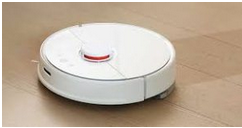
\includegraphics[width=\textwidth, height=\textwidth]{roomba.png}
    \caption{Roomba}
  \end{subfigure}
    \hfill
  \begin{subfigure}[b]{0.3\textwidth}
    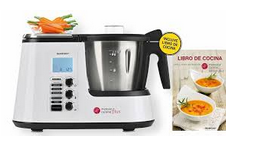
\includegraphics[width=\textwidth, height=\textwidth]{thermomix.png}
    \caption{Thermomix}
  \end{subfigure}
      \hfill
  \begin{subfigure}[b]{0.3\textwidth}
    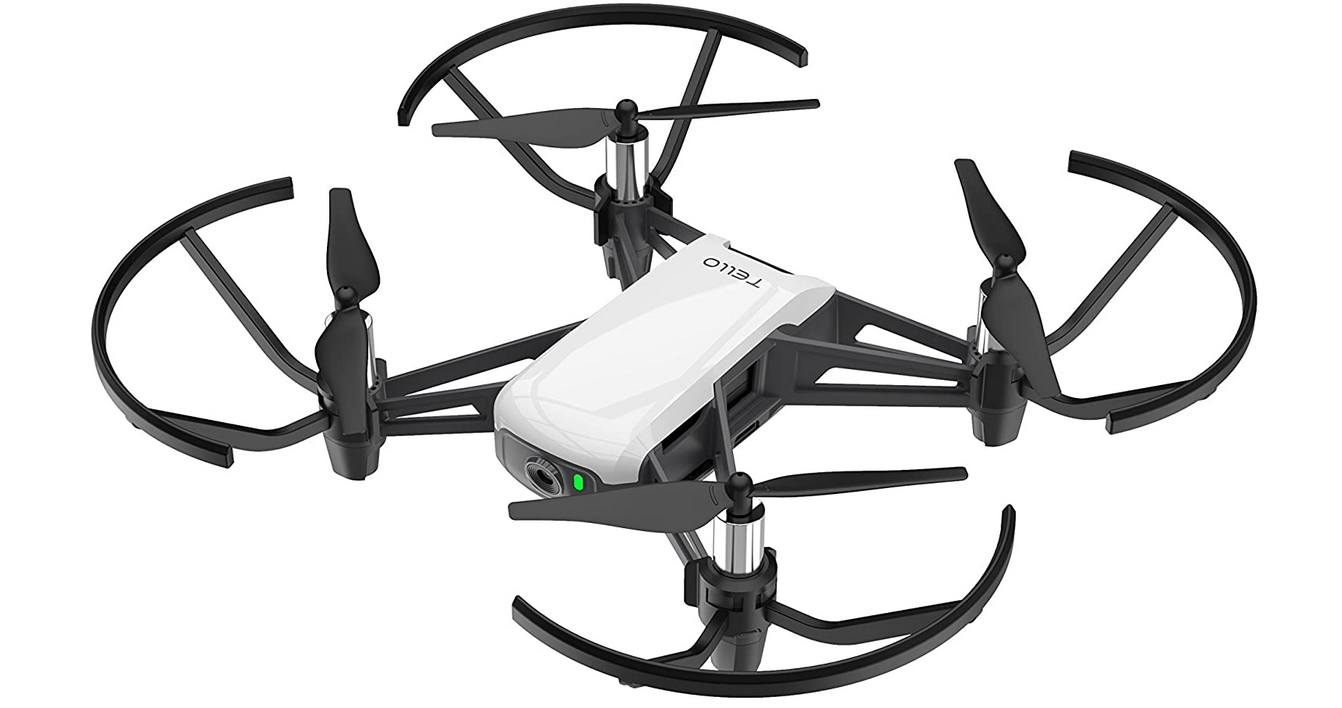
\includegraphics[width=\textwidth, height=\textwidth]{drone.png}
    \caption{Tello}
  \end{subfigure}
      \hfill
  \begin{subfigure}[b]{0.3\textwidth}
    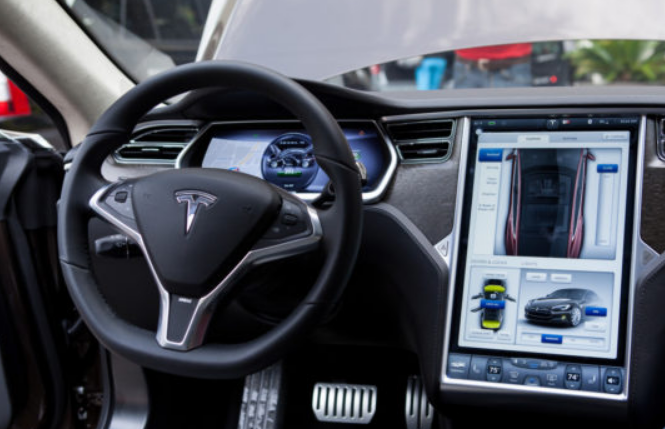
\includegraphics[width=\textwidth, height=\textwidth]{tesla.png}
    \caption{Tesla}
  \end{subfigure}
        \hfill
  \begin{subfigure}[b]{0.3\textwidth}
    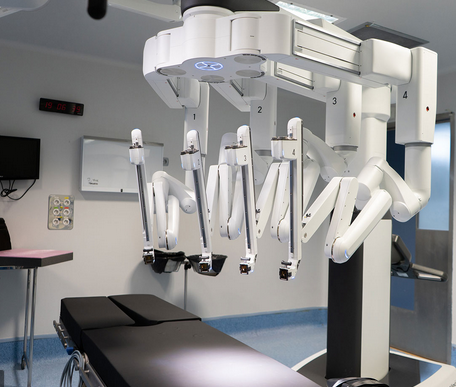
\includegraphics[width=\textwidth, height=\textwidth]{davinci.png}
    \caption{Robot DaVinci}
  \end{subfigure}
        \hfill
  \begin{subfigure}[b]{0.3\textwidth}
    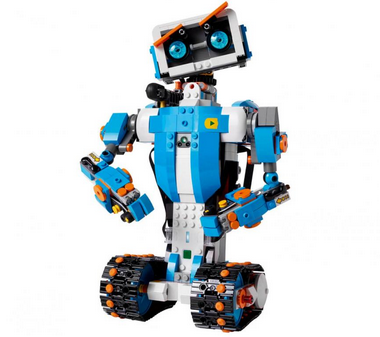
\includegraphics[width=\textwidth, height=\textwidth]{lego.png}
    \caption{Robots LEGO}
  \end{subfigure}
\caption{Ejemplos de robots en la actualidad}
\label{fig:EjemplosRobots}
\end{figure}


\section{Tecnologías web}
Las tecnologías web están en continuo desarrollo. Actualmente, existen tecnologías webtanto en el lado del cliente como en el lado del servidor. La idea de esta separación es marcar las diferentes partes de un sistema software para poder controlarlo de una forma más eficaz. Por este motivo, el \textit{frontend} recoge los datos y el \textit{backend} los procesa. \newline

Hoy en día, son muy comunes las aplicaciones web que se basan en estas tecnologías. Las aplicaciones web basan su funcionamiento en un modelo cliente - servidor en el que el cliente se encarga de recoger los datos que introduce el usuario y el servidor los procesa. Algunas de las aplicaciones web con más éxito en los últimos años son \textit{Gmail}, \textit{Spotify}, \textit{Netflix}, \textit{Amazon} o \textit{AliExpress}.

\begin{figure}[!h]
  \begin{subfigure}[b]{0.5\textwidth}
    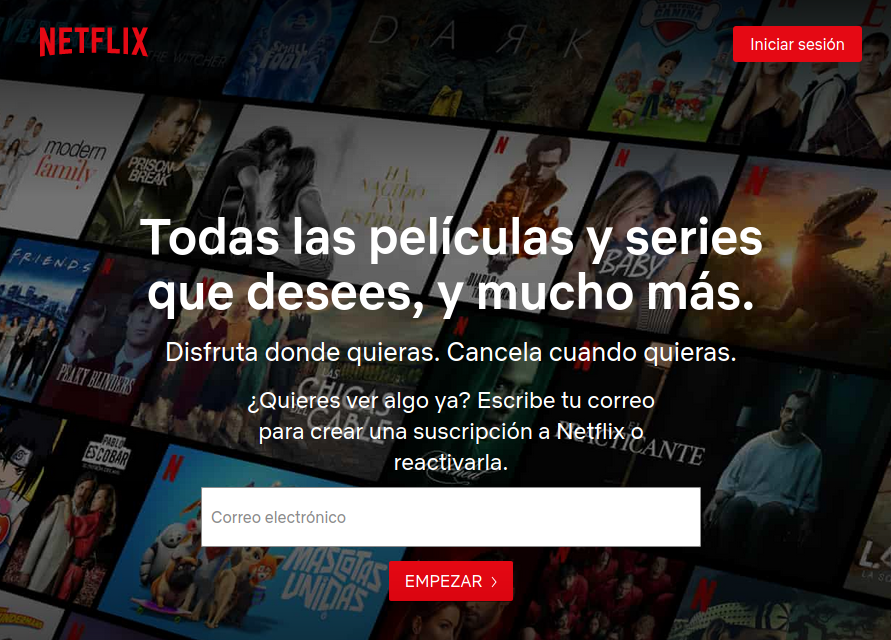
\includegraphics[width=\textwidth, height=\textwidth]{netflix.png}
    \caption{Aplicación web dedicada a la distribución de contenidos}
  \end{subfigure}
        \hfill
  \begin{subfigure}[b]{0.5\textwidth}
    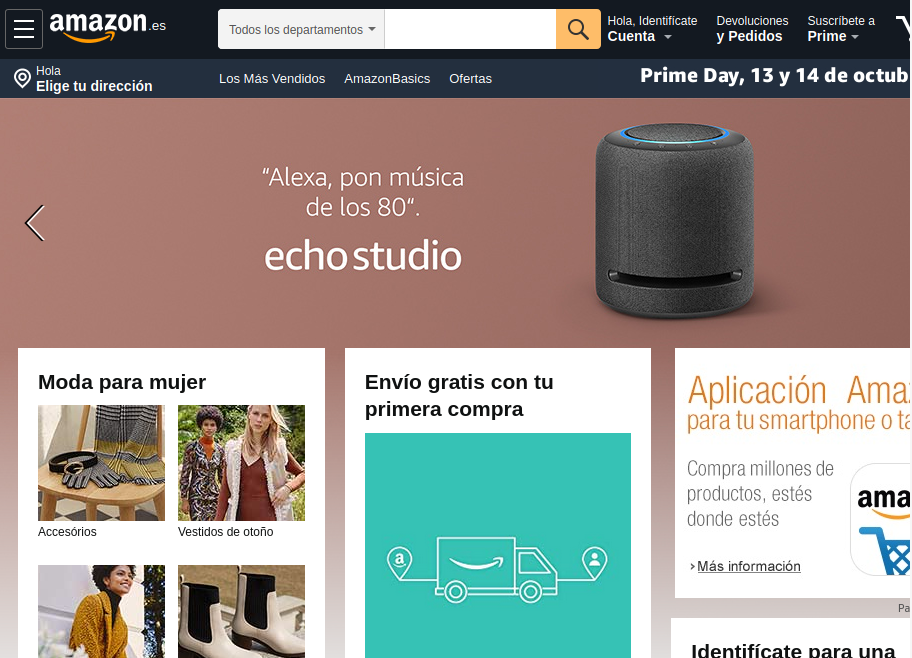
\includegraphics[width=\textwidth, height=\textwidth]{amazon.png}
    \caption{Aplicación web dedicada a la venta online}
  \end{subfigure}
\caption{Ejemplos de aplicaciones web}
\label{fig:ejemplosaplicaciones}
\end{figure}

Por un lado, el \textit{frontend} engloba todas aquellas tecnologías web del lado del cliente que se encargan de recopilar los datos y mostrárselos al usuario. Principalmente, existen tres tecnologías de \textit{frontend}: \textit{HTML, CSS} y \textit{JavaScript}. Estas tres tecnologías permiten al usuario interactuar con el sevidor web, utilizando un navegador como intérprete. \newline 

Por otro lado, el \textit{backend} se encarga del almacenamiento de información en bases de datos, gestión de servidores y servir las vistas de las páginas web seleccionadas por el desarrollador en el lado del cliente. En el backend, el número de tecnologías es mucho más extenso. La programación \textit{backend} incluye lenguajes como \textit{PHP, Python, .NET o Java }y las bases de datos sobre las que se trabaja pueden ser \textit{SQL, MongoDB o MySQL}. \newline 

La comunicación entre cliente y servidor se realiza utilizando el protocolo \textit{HTTP} (protocolo de transferencia de hipertexto). Este protocolo funciona mediante la emisión de una serie de peticiones y respuestas entre el cliente y el servidor usando diferentes métodos. Existen numerosos métodos \textit{HTTP}, pero los más comunes son los siguientes\footnote{https://developer.mozilla.org/es/docs/Web/HTTP/Methods}:

\begin{itemize}
    \item \textbf{GET}: solicitud de datos de un recurso concreto.
    \item \textbf{PUT}: reemplazo de las representaciones actuales del recurso de la petición.
    \item \textbf{POST}: envío de datos a un recurso concreto, normalmente provocando el cambio de estado del servidor.
    \item \textbf{DELETE}: eliminación de un recurso.
     \item \textbf{HEAD}: solicitud de datos de un recurso concreto tal y como ocurre con el método \textit{GET}, pero la respuesta no incluye cuerpo.
\end{itemize}

\begin{figure}[h!]
    \centering
    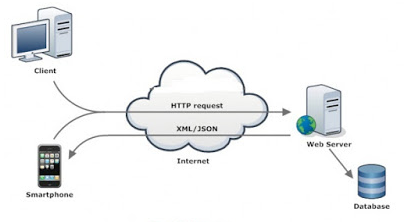
\includegraphics[scale=1]{http.png}
    \caption{Ejemplo de una interacción \textit{HTTP} \footnotemark}
    \label{fig:http}
\end{figure}
\footnotetext{http://dsanchezzz.blogspot.com/2015/10/rest.html}
\subsection{Tecnologías web en el lado del cliente}
Las tres tecnologías web del frontend que permiten la interacción entre usuario y servidor web son las siguientes:
\begin{itemize}
    \item \textit{HTML:} es un lenguaje de marcado que permite diferenciar los contenidos y definir la estructura de un sitio web. Permite dividir una página web en diferentes secciones: títulos, texto, imágenes, pie de página, etc. Es la base de toda página web. Sigue el modelo de objetos \textit{Document Object Model (DOM)}, que permite que el contenido de una página esté disponible para los programas en \textit{JavaScript}. Hoy en día, los navegadores emplean la versión \textit{HTML5}, que introduce como mejora las etiquetas de vídeo, de audio, de diálogos entre personas, de secciones y de bloques de contenidos.
    \item \textit{CSS}: es un lenguaje de hojas de estilo que permite modificar la apariencia de una página web. Gracias a este lenguaje, se puede organizar mejor el código al poder separar los datos (lenguaje \textit{HTML}) del diseño (lenguaje \textit{CSS}). Hoy en día, la versión disponible en los navegadores en \textit{CSS3}.
    \item \textit{JavaScript:} es un lenguaje de programación interpretado que permite definir el comportamiento de una página web (por ejemplo, al hacer click en un enlace). Por ello, gracias a este lenguaje el usuario puede interaccionar con la página web.
\end{itemize}

\subsection{Tecnologías web en el lado del servidor}
En el lado del servidor, algunas de las tecnologías que permiten acceder a bases de datos, escalabilidad, gestionar los servidores y servir las páginas web mediante la utilización de plantillas son:

\begin{itemize}
    \item \textit{Node.js}: uno de los lenguajes frecuentemente utilizado en la programación del \textit{backend} es el lenguaje \textit{JavaScript}. \textit{JavaScript} se creó para su uso en el \textit{frontend} en un principio; sin embargo, gracias al motor \textit{node.js}, este lenguaje puede ser interpretado en el lado del servidor sin necesidad de un navegador.
    \item \textit{Django}: es un entorno web de alto nivel programado en \textit{Python}. Es muy rápido y fácil de utilizar. Además, dispone de una interfaz para el manejo de las bases de datos \textit{SQL} y se puede acceder a ellas en el código mediante instrucciones \textit{Python}.
    \item \textit{Java}: es un lenguaje de programación y una plataforma informática empleada en un gran número de aplicaciones y sitios web. Es rápido, fiable y escalable. Su lenguaje deriva del de \textit{C} y \textit{C++}, pero con un nivel de abstracción más alto.
\end{itemize}


\section{Docencia robótica}
Las tecnologías web ofrecen nuevas posibilidades para la robótica. Una de estas posibilidades es la docencia robótica. La docencia robótica ha estado creciendo en los últimos años gracias a que se trata de un campo de gran utilidad y que es una manera atractiva y divertida de introducir a los niños en la tecnología. Hoy en día existen muchas iniciativas para promover la docencia robótica. De hecho, ya se ha introducido en el currículum oficial de secundaria en muchas comunicades autónomas de España y en otros países del mundo.  \newline

En consecuencia, especialmente en los últimos años, han surgido algunas plataformas dedicadas a la docencia robótica que se encargan de impartir cursos de iniciación a la robótica desde edades muy tempranas para conseguir que los niños se sientan atraídos por esta rama desde el principio y aprendan a pensar como verdaderos programadores desde muy pequeños. \newline

La docencia robótica comparte los fundamentos de la educación \textit{STEM (Science, Technology, Engineering and Mathematics)}. Esta educación promueve el aprendizaje de la ciencia, tecnología, ingeniería y matemáticas y fomenta el desarrollo de un pensamiento crítico y la creatividad. \newline

Un ejemplo de estas plataformas que se comentan es el de \textit{Lenobotics}\footnote{https://lenobotics.com/}.  \textit{Lenobotics} es un programa que se encarga de impartir cursos de robótica en centros educativos para desarrollar las habilidades cognitivas de los niños que resultan necesarias para la programación. \newline

\clearpage
\begin{figure}[h!]
    \centering
    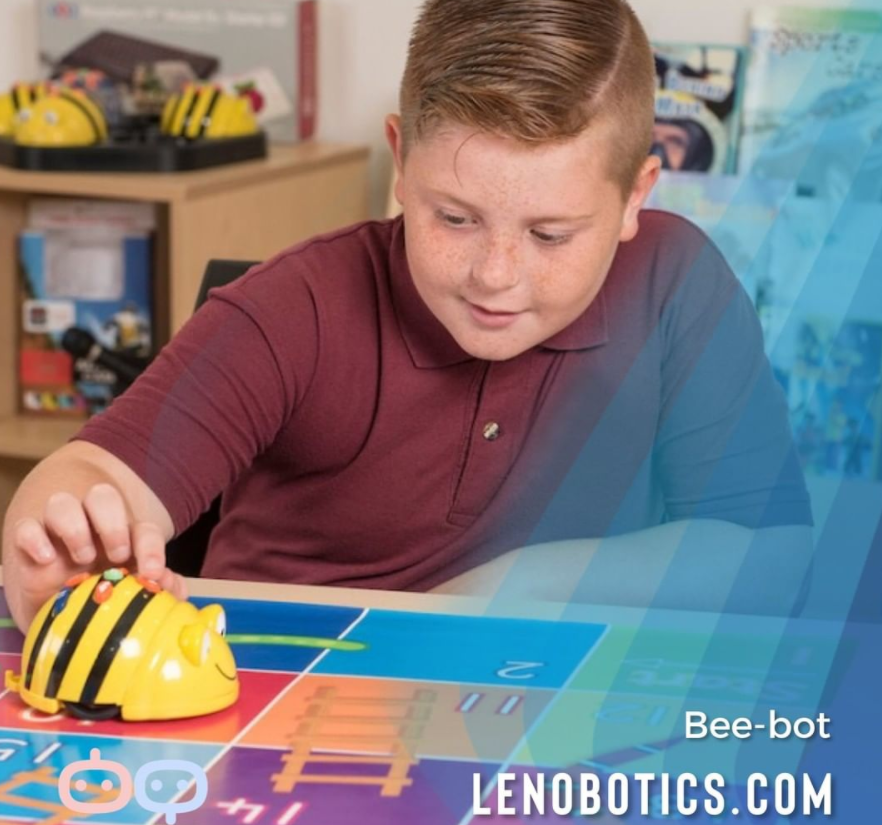
\includegraphics[scale=0.55]{lenobotics.PNG}
    \caption{Aprendizaje de programación robótica con \textit{Lenobotics}}
    \label{fig:lenobotics}
\end{figure}


Por su parte, \textit{LEGO education}\footnote{https://education.lego.com/es-es} también ofrece a los más pequeños la posibilidad de iniciarse en la robótica a través de sus kits. Estos kits permiten aprender unas primeras nociones de electrónica, robótica y programación. \newline

\begin{figure}[h!]
    \centering
    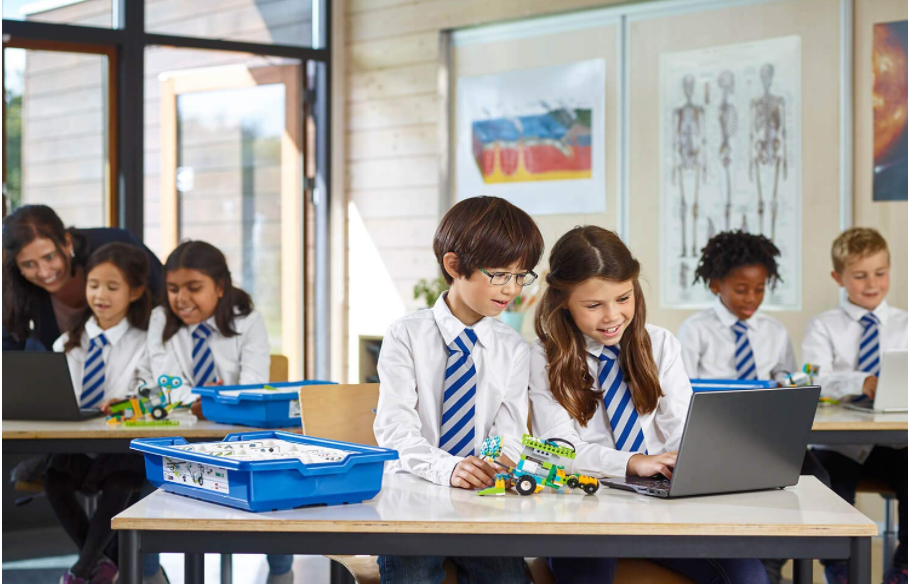
\includegraphics[scale=0.7]{lego.PNG}
    \caption{Aprendizaje de programación robótica con \textit{LEGO education}}
    \label{fig:lego}
\end{figure}

\clearpage
Otro ejemplo es el de \textit{OpenRoberta}\footnote{https://lab.open-roberta.org/}, que ofrece una interfaz de programación por medio de bloques de texto para diferentes modelos de robot. También dispone de una sección con ejercicios resueltos de muestra, para que los más inexpertos puedan empezar a familiarizarse con ellos.

\begin{figure}[h!]
    \centering
    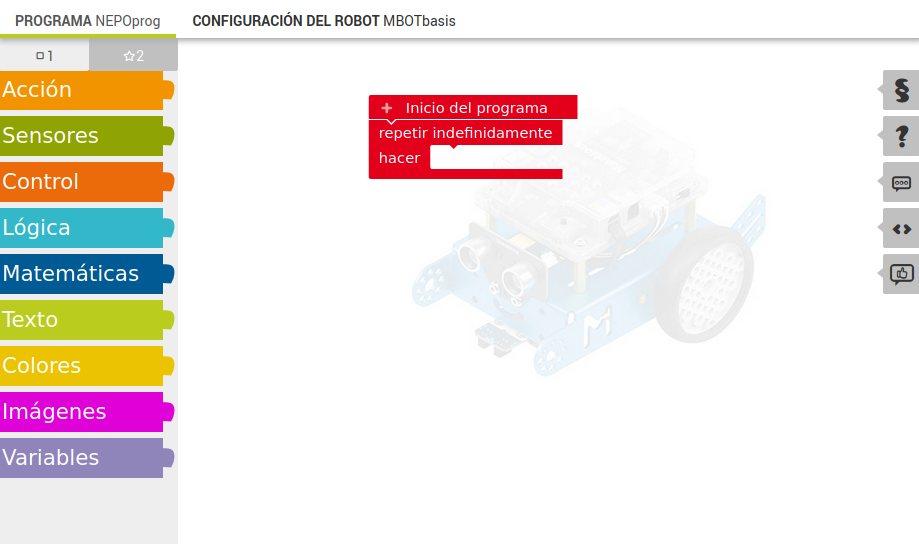
\includegraphics[scale=0.5]{openroberta.PNG}
    \caption{Aprendizaje de programación robótica con \textit{OpenRoberta}}
    \label{fig:lego}
\end{figure}

\textit{iRobot}\footnote{https://edu.irobot.com/} ofrece la posibilidad tanto de crear modelos de robot como de programar el cerebro de esos robots. Este entorno hace especial hincapié en la enseñanza \textit{STEM} como mejor método de aprendizaje de robótica.

\clearpage

\begin{figure}[h!]
    \centering
    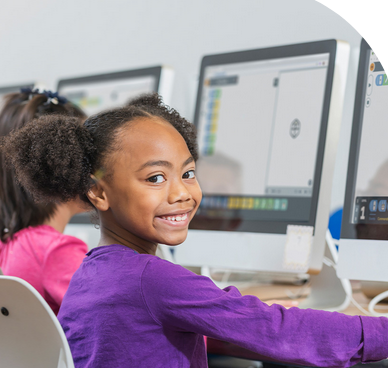
\includegraphics[scale=0.7]{irobot.PNG}
    \caption{Aprendizaje de programación robótica con \textit{iRobot}}
    \label{fig:lego}
\end{figure}

El presente trabajo se va a centrar en la plataforma \textit{Kibotics}\footnote{https://kibotics.org/}. \textit{Kibotics} es un entorno web para docencia en robótica y programación que permite a niños y adolescentes aprender programando. Esto quiere decir que \textit{Kibotics}  apuesta por una enseñanza principalmente práctica, ya que resulta mucho más atractiva tanto la enseñanza como el aprendizaje de este modo que únicamente con clases teóricas. \newline

\textit{Kibotics}  se basa en la utilización del simulador \textit{WebSim}  que, a su vez, está basado en la tecnología \textit{A-Frame}  para representar los mundos. Este simulador permite la creación de diferentes ejercicios para los robots que tienen soporte en la plataforma: piBot, mBot, fórmula 1 y drone Tello. Estos ejercicios podrán solucionarse tanto en \textit{Scratch} (especialmente indicado para aquellos alumnos que no hayan programado anteriormente) como en \textit{Python} (para aquellos niños que cuenten con nociones previas). \newline

\begin{figure}[h!]
    \centering
    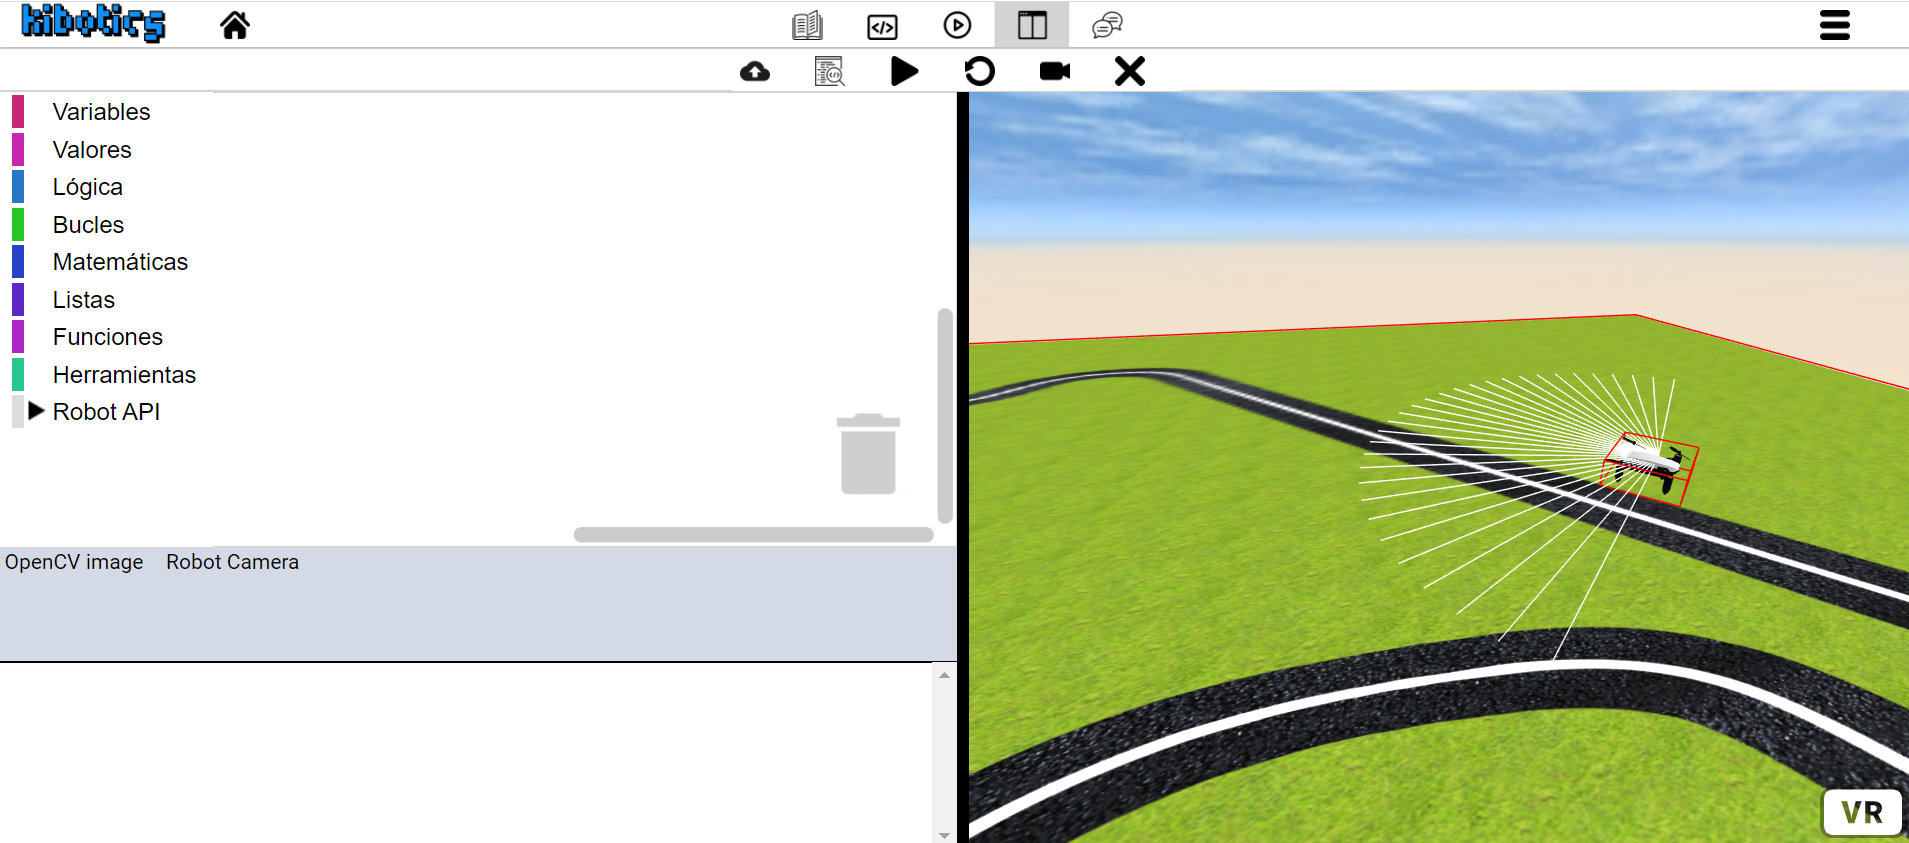
\includegraphics[scale=0.5]{kibotics.PNG}
    \caption{Interfaz de programación en \textit{Kibotics} de un ejercicio en \textit{Scratch}}
    \label{fig:kibotics}
\end{figure}


Todos los robots cuentan con cámaras incorporadas en el hardware, lo que permite la creación de ejercicios que se deben solucionar mediante la utilización de la visión artificial además de los ejercicios que se puedan solucionar mediante el uso de los sensores de los robots (sensores infrarrojos, por ejemplo). La Figura \ref{fig:RobotsKibotics} muestra los robots que soporta actualmente la plataforma.\newline


\begin{figure}[h!]
  \begin{subfigure}[b]{0.2\textwidth}
    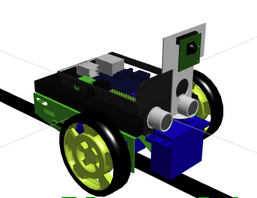
\includegraphics[width=\textwidth, height=\textwidth]{pibot.png}
    \caption{piBot}
  \end{subfigure}
  \hfill
  \begin{subfigure}[b]{0.2\textwidth}
    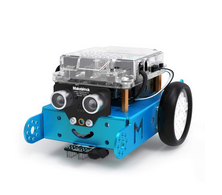
\includegraphics[width=\textwidth, height=\textwidth]{mbot.png}
    \caption{mBot}
  \end{subfigure}
    \hfill
  \begin{subfigure}[b]{0.2\textwidth}
    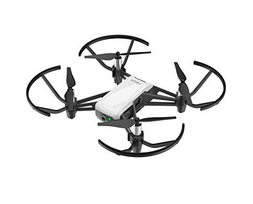
\includegraphics[width=\textwidth, height=\textwidth]{tello_2.png}
    \caption{Drone Tello}
  \end{subfigure}
    \hfill
  \begin{subfigure}[b]{0.2\textwidth}
    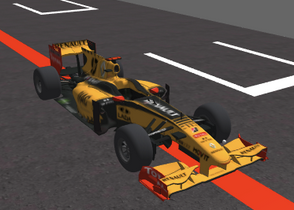
\includegraphics[width=\textwidth, height=\textwidth]{f1.png}
    \caption{Fórmula 1}
  \end{subfigure}
\caption{Robots soportados en la plataforma \textit{Kibotics}}
\label{fig:RobotsKibotics}
\end{figure}


Por último, cabe destacar la importancia de los motores de físicas que incorporan los simuladores robóticos usados tanto en docencia como en investigación robótica. Un motor de físicas es un software capaz de realizar simulaciones de ciertos sistemas físicos como la dinámica del cuerpo en movimiento, la fricción y la elasticidad de una colisión. Se emplean con mucha frecuencia en los videojuegos, para recrear con un mayor realismo el movimiento de los personajes. \newline

Existen numerosos motores de físicas como \textit{Box2D}\footnote{https://box2d.org/} (simulaciones 2D), \textit{Cocos2D,}\footnote{https://www.cocos.com/} (simulaciones 2D) \textit{Ammo.js}\footnote{https://github.com/kripken/ammo.js/} (simulaciones 3D) o \tetxit{CANNON}\footnote{http://schteppe.github.io/cannon.js/} (simulaciones 3D). El presente trabajo se va a centrar en este último, ya que es el que emplea \textit{A-Frame} en la actualidad. \\ En el capítulo 3, se explicará con mayor detalle las peculiaridades de este motor de físicas en cuestión. 

